\documentclass[a4paper,12pt,twoside,spanish]{book}
% Inicialización del documento

% Paquetes
\usepackage [spanish]{babel}
\usepackage[utf8]{inputenc}
\selectlanguage{spanish}
\usepackage[dvips]{graphicx}
\usepackage[colorlinks=true,linkcolor=black]{hyperref}
\usepackage{amsmath}
\usepackage{amsfonts}
\usepackage{mathptmx} % Times New Roman en LaTeX
\usepackage{amssymb}
\usepackage{anysize}
\usepackage{latexsym}
\usepackage{epsfig}
\usepackage{fancyhdr}
\usepackage{float}
\usepackage{colortbl}
\usepackage{color}
\usepackage{wrapfig}
\usepackage{subfigure}
\usepackage{epstopdf}
\usepackage{booktabs}
\usepackage[T1]{fontenc}
\usepackage[outermargin=-2.5cm,]{fullwidth}
\usepackage{boxedminipage}
\usepackage{shadow}
\usepackage{lscape}
\usepackage{titlesec}
\usepackage{curves}
\usepackage{rotating}
\usepackage{calc}
\usepackage{url}
\usepackage{babelbib}
\usepackage{hyperref}
\hypersetup{
   citecolor=black
}
\usepackage[justification=centering]{caption}
\usepackage{setspace}
\usepackage{nomencl}
\makenomenclature
\usepackage[nottoc]{tocbibind} % Para que aparezcan la tabla de figuras y cuadros en el índice
\renewcommand{\nomname}{Lista de acrónimos y abreviaturas}


\usepackage{listings}
\usepackage{xcolor}

\definecolor{codegreen}{rgb}{0,0.6,0}
\definecolor{codegray}{rgb}{0.5,0.5,0.5}
\definecolor{codepurple}{rgb}{0.58,0,0.82}
\definecolor{backcolour}{rgb}{0.95,0.95,0.92}

\lstdefinestyle{mystyle}{
	backgroundcolor=\color{backcolour},   
	commentstyle=\color{codegreen},
	keywordstyle=\color{magenta},
	numberstyle=\tiny\color{codegray},
	stringstyle=\color{codepurple},
	basicstyle=\ttfamily\footnotesize,
	breakatwhitespace=false,         
	breaklines=true,                 
	captionpos=b,                    
	keepspaces=true,                 
	numbers=left,                    
	numbersep=5pt,                  
	showspaces=false,                
	showstringspaces=false,
	showtabs=false,                  
	tabsize=2
}
\lstset{style=mystyle}

% Paquetes

% Formato de las páginas
\onehalfspace 
\raggedbottom
\pagestyle{fancy} 
\addtolength{\headwidth}{\marginparsep}
\setlength{\headheight}{25pt}
\setlength{\oddsidemargin}{0cm}
\setlength{\evensidemargin}{0cm}
\marginsize{2.5cm}{2.5cm}{2.5cm}{2.5cm}
\fancyhf{}
\fancyhead[LE,RO]{\bfseries \thepage} 
\fancyhead[LO]{\sffamily\scshape\footnotesize\rightmark} 
\fancyhead[RE]{\sffamily\scshape\footnotesize\leftmark} 
\addtolength{\parskip}{5pt}
% Formato de las páginas

\begin{document}
\chapter{Análisis script meshAP.py}
\section{Configuración del script meshAP.py}

Este fichero contiene la configuración de una red mesh simple que cuenta con dos access points y dos estaciones base. Dicha configuración corresponde a la de una red SDN en la que los access points funcionan como switches típicos de este tipo de redes.\par

El contenido del script meshAP.py es el siguiente: \par

\begin{lstlisting}
#!/usr/bin/python

'''
This example shows on how to create wireless link between two APs 
with mesh
The wireless mesh network is based on IEEE 802.11s
'''

from mininet.log import setLogLevel, info
from mn_wifi.link import wmediumd, mesh
from mn_wifi.cli import CLI
from mn_wifi.net import Mininet_wifi
from mn_wifi.wmediumdConnector import interference


def topology():
'Create a network.'
net = Mininet_wifi(link=wmediumd, wmediumd_mode=interference)

info('*** Creating nodes\n')
sta1 = net.addStation('sta1', mac='00:00:00:00:00:11', 
	position='1,1,0')
sta2 = net.addStation('sta2', mac='00:00:00:00:00:12', 
	position='31,11,0')
ap1 = net.addAccessPoint('ap1', wlans=2, ssid='ssid1', 
	position='10,10,0')
ap2 = net.addAccessPoint('ap2', wlans=2, ssid='ssid2', 
	position='30,10,0')
c0 = net.addController('c0')

info('*** Configuring wifi nodes\n')
net.configureWifiNodes()

info('*** Associating Stations\n')
net.addLink(sta1, ap1)
net.addLink(sta2, ap2)
net.addLink(ap1, intf='ap1-wlan2', cls=mesh, ssid='mesh-ssid', 
	channel=5)
net.addLink(ap2, intf='ap2-wlan2', cls=mesh, ssid='mesh-ssid', 
	channel=5)

info('*** Starting network\n')
net.build()
c0.start()
ap1.start([c0])
ap2.start([c0])

info('*** Running CLI\n')
CLI(net)

info('*** Stopping network\n')
net.stop()


if __name__ == '__main__':
setLogLevel('info')
topology()
\end{lstlisting}

Se trata de una red mesh de medio inalámbrico \
($link=wmedium$) con interferencias ($wmedium\_mode=interference$). El simulador se encarga de calcular el nivel de interferencia en base a la distancia existente entre un nodo y sus nodos adyacentes. También se desprende del script que la red presenta el controlador propio de las redes definidas por software, conocidas como redes SDN por sus siglas en inglés.\par

Los dos puntos de acceso (\textit{access points} (APs) en adelante) de la red mesh configurada en el script presentan cada uno de ellos dos WLANs, una de ellas con configuración mesh. Además se indica las direcciones MAC de las dos estaciones base \textit{sta1} y \textit{sta2}.\par

Respecto a los enlaces entre los diferentes nodos de la red, se observa que se configura un enlace entre \textit{ap1} y \textit{ap1} y otro entre \textit{sta2} y \textit{ap2}. En \textit{ap1} y \textit{ap2} además se configuran las interfaces 'ap1-wlan2' y 'ap2-wlan2' como enlaces mesh en el canal 5 de la red.\par








\section{Topología inicial}\label{sect:topo_inicial}

En la Figura \ref{fig:pos} se representa la posición de los nodos y APs de la red, obtenida mediante el módulo de representación que ofrece el entorno Mininet Wifi.

	\begin{figure}[!h]
		\centering
		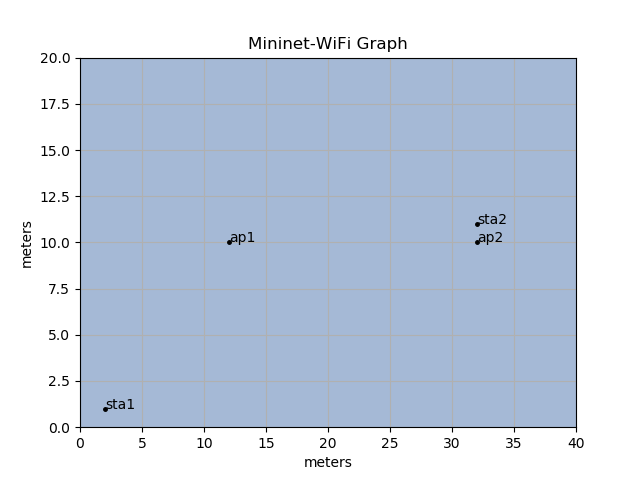
\includegraphics[scale=0.7]{Figuras/posicion.png}
		\caption{Posición de los nodos de la red meshAP.}
		\label{fig:pos}
	\end{figure}

Con la información que se tiene hasta el momento (la que aporta el script meshAP.py y la posición de los equipos de la red), se puede determinar que la topología de la red mesh es la indicada en la Figura \ref{fig:topo_inicial}, a falta de conocer cuáles son las interfaces que se conectan entre los diferentes equipos.\par

	\begin{figure}[!h]
		\centering
		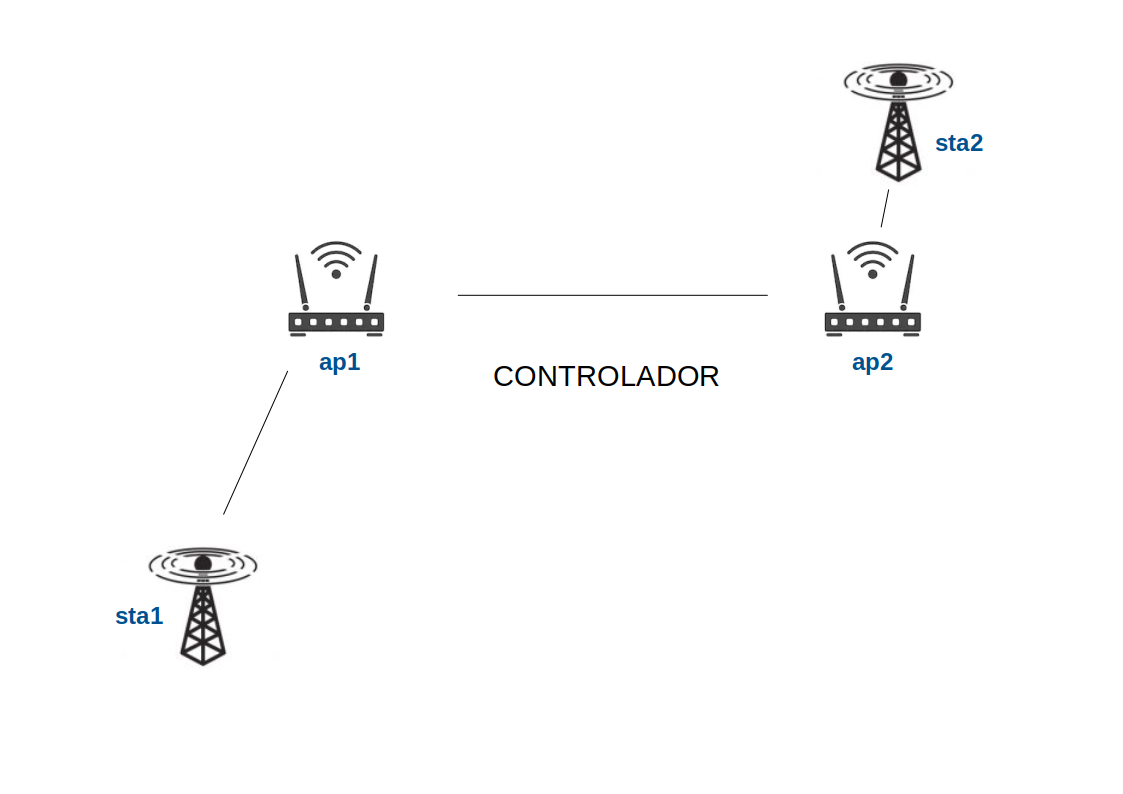
\includegraphics[scale=.4]{Figuras/topo_inicial.png}
		\caption{Topología de la red meshAP.}
		\label{fig:topo_inicial}
	\end{figure}

Sin embargo, aún falta conocer cuáles son las interfaces de los nodos, cómo se conectan entre ellas y qué papel tiene en estas conexiones el controlador de la red. En los siguientes apartados del presente capítulo se analizará el funcionamiento de la red en ejecución para comprender cómo funciona realmente una red mesh definida por software y poder completar el esquema de la topología de la red analizada.\par







\section{Establecimiento de la conexión y configuración de las interfaces}







\section{Análisis de los flujos de datos con \texttt{pingall}}\label{sect:tablas_flujos}


Hay que recordar que el comando \texttt{pingall} se encarga de ejecutar un mensaje \textit{ping} entre todas las estaciones base que componen una red. En la red meshAP, por tanto, se generarán 2 \textit{pings}: uno desde sta1 hacia sta2, y otro en el sentido contrario.\par

Los mensajes \textit{ping} funcionan de la siguiente manera: la estación origen envía un paquete \texttt{ICMP echo request} hacia la estación destino, que debe contestar con otro mensaje \texttt{ICMP echo reply}. Si la estación base origen no conoce la dirección MAC de la estación destino, además se generan mensajes \texttt{ARP request} y \texttt{ARP reply}. En el \texttt{ARP request}, la estación origen envía el mensaje a todos los nodos (estaciones base, puntos de acceso, \textit{hosts}) a los que se encuentra conectada, es decir, lo envía a la dirección de broadcast (ff:ff:ff:ff:ff:ff). En este mensaje, origen pregunta quién tiene la dirección IP destino del \texttt{ICMP echo request}, y el nodo al que pertenezca dicha IP responde con su dirección MAC en un mensaje \texttt{ARP reply} a la estación origen. Una vez conocida la dirección MAC del destino, el origen envía el \texttt{ICMP echo request}. Cuando el destino lo recibe, puede ocurrir que tampoco tenga la dirección MAC del origen, si se ha borrado de su caché, por lo que tendría que realizar el mismo procedimiento con los mensajes ARP para conocerla y, finalmente, enviar su respuesta ICMP echo reply a esa dirección.\par

Sin embargo, en las redes SDN el proceso de mensajes se ve un poco alterado. Cuando sta1 envía su \texttt{ARP request} hacia la dirección de broadcast para conocer la dirección MAC de sta2, en primer lugar el mensaje llega al \textit{access point} ap1. Seguidamente, ap1 deberá consultar su tabla de flujos para comprobar si existe alguna entrada para tráfico \texttt{ARP request} procedente de sta1 y destinado a sta2. Si tiene alguna entrada que coincida para este tipo de tráfico, sigue las normas o acciones que se indiquen en ella. Si por el contrario, no la tiene, deberá consultar al controlador de la red qué debe hacer en ese caso.\par 

Entre los \textit{access points} y el controlador de una red SDN se intercambian distintos tipos de mensajes. Normalmente el \textit{access point} consulta qué hacer y el controlador le indica a quién debe enviar el tráfico, por qué puerto, si debe eliminarlo, o si tiene que añadir una nueva entrada para ese tipo de tráfico en su tabla de flujos. Estos mensajes entre el controlador y los \textit{access points} se analizan con más detalle en el Apartado \ref{sect:capt_of} del presente capítulo.\par 

A continuación se analiza el contenido de las tablas de flujos del controlador c0 de la red, y de los puntos de acceso ap1 y ap2. Como se ha indicado, estas tablas deberían tener entradas para todos los tipos de tráfico que se envían entre los nodos, tras ejecutar el comando \texttt{pingall}.\par 

\hspace{0.5cm}

El datapath del controlador de la red tiene los siguientes puertos e interfaces:
\texttt{\\
\noindent system@ovs-system:\\
	\indent lookups: hit:79 missed:37 lost:0\\
	\indent	flows: 0\\
	\indent	masks: hit:153 total:0 hit/pkt:1.32\\
	\indent	port 0: ovs-system (internal)\\
	\indent	port 1: ap1-wlan1\\
	\indent	port 2: ap1-wlan2\\
	\indent	port 3: ap1-mp2\\
	\indent	port 4: ap1 (internal)\\
	\indent	port 5: ap2-wlan1\\
	\indent	port 6: ap2-wlan2\\
	\indent	port 7: ap2-mp2\\
	\indent	port 8: ap2 (internal)\\
}\par

Para comprobar los flujos que se instalan en el controlador, se debe ejecutar el siguiente comando:\par 

\begin{center} 
	\texttt{mininet-wifi> sh ovs-dpctl dump-flows}
\end{center}

\noindent\texttt{
	recirc\_id(0),in\_port(5),eth(src=00:00:00:00:00:12,dst=00:00:00:00:00:11),
	eth\_type(0x0800),ipv4(src=10.0.0.2,dst=10.0.0.1,proto=1,tos=0/0xfc,frag=no),
	icmp(type=8,code=0), packets:0, bytes:0, 	used:never, actions:7
}

Regla 1: indica que todo el tráfico ICMP ECHO (icmp\_type=8, icmp\_code=0) que entre por el puerto 5 del controlador (interfaz ap2-wlan1), con direcciones MAC origen y destino 00:00:00:00:00:12 y 00:00:00:00:00:11, respectivamente, y direcciones IP 10.0.0.2 y 10.0.0.1, origen y destino, salga por el puerto 7, interfaz ap2-mp2.\par 

\noindent\texttt{
	recirc\_id(0),in\_port(7),eth(src=00:00:00:00:00:11,dst=00:00:00:00:00:12),
	eth\_type(0x0800),ipv4(src=10.0.0.1,dst=10.0.0.2,proto=1,tos=0/0xfc,frag=no),
	icmp(type=0,code=0), packets:0, bytes:0, 	used:never, actions:5
}

Regla 2: indica que todo el tráfico ICMP echo reply (icmp\_type=0, icmp\_code=0) que entre por el puerto 7 del controlador (interfaz ap2-mp2), con direcciones MAC origen y destino 00:00:00:00:00:11 y 00:00:00:00:00:12, respectivamente, y direcciones IP 10.0.0.1 y 10.0.0.2, origen y destino, salga por el puerto 5, interfaz ap2-wlan1.\par 

\noindent\texttt{
	recirc\_id(0),in\_port(3),eth(src=00:00:00:00:00:12,dst=00:00:00:00:00:11),
	eth\_type(0x0800),ipv4(src=10.0.0.2,dst=10.0.0.1,proto=1,tos=0/0xfc,frag=no),
	icmp(type=8,code=0), packets:0, bytes:0, 	used:never, actions:1
}

Regla 3: indica que todo el tráfico ICMP ECHO (icmp\_type=8, icmp\_code=0) que entre por el puerto 3 del controlador (interfaz ap1-mp2), con direcciones MAC origen y destino 00:00:00:00:00:12 y 00:00:00:00:00:11, respectivamente, y direcciones IP 10.0.0.2 y 10.0.0.1, origen y destino, salga por el puerto 1, interfaz ap1-wlan1.\par 


\noindent\texttt{
	recirc\_id(0),in\_port(1),eth(src=00:00:00:00:00:11,dst=00:00:00:00:00:12),
	eth\_type(0x0800),ipv4(src=10.0.0.1,dst=10.0.0.2,proto=1,tos=0/0xfc,frag=\\no),
	icmp(type=0,code=0), packets:0, bytes:0, 	used:never, actions:3
}

Regla 4: indica que todo el tráfico ICMP echo reply (icmp\_type=0, icmp\_code=0) que entre por el puerto 1 del controlador (interfaz ap1-wlan1), con direcciones MAC origen y destino 00:00:00:00:00:11 y 00:00:00:00:00:12, respectivamente, y direcciones IP 10.0.0.1 y 10.0.0.2, origen y destino, salga por el puerto 3, interfaz ap1-mp2.\par 

\noindent\texttt{
	recirc\_id(0),in\_port(3),eth(src=00:00:00:00:00:12,dst=00:00:00:00:00:11),
	eth\_type(0x0806),arp(sip=10.0.0.2,tip=10.0.0.1,
	op=1/0xff), packets:0,\\
	bytes:0, used:never, actions:1
}

Regla 5: indica que todo el tráfico ARP request (op=1) que entre por el puerto 3 del controlador (interfaz ap1-mp2), con direcciones MAC origen y destino 00:00:00:00:00:12 y 00:00:00:00:00:11, respectivamente, y direcciones IP 10.0.0.2 y 10.0.0.1, origen y destino, salga por el puerto 1, interfaz ap1-wlan1.\par

\noindent\texttt{
	recirc\_id(0),in\_port(5),eth(src=00:00:00:00:00:12,dst=00:00:00:00:00:11),
	eth\_type(0x0806),arp(sip=10.0.0.2,tip=10.0.0.1,op=1/0xff), packets:0, \\
	bytes:0, used:never, actions:7
}

Regla 6: indica que todo el tráfico ARP request (op=1) que entre por el puerto 5 del controlador (interfaz ap2-wlan1), con direcciones MAC origen y destino 00:00:00:00:00:12 y 00:00:00:00:00:11, respectivamente, y direcciones IP 10.0.0.2 y 10.0.0.1, origen y destino, salga por el puerto 7, interfaz ap2-mp2.\par 

\hspace{1cm}

Para ver la tabla de flujos del \textit{access point} ap1, hay que ejecutar el siguiente comando:\par 

\begin{center}
	\texttt{mininet-wifi> sh ovs-ofctl dump-flows ap1}
\end{center}

\noindent\texttt{
	cookie=0x0, duration=5.054s, table=0, n\_packets=0, n\_bytes=0, idle\_timeout\\
	=60, priority=65535, arp,
	in\_port='ap1-mp2',vlan\_tci=0x0000,dl\_src=00:00:00:\\
	00:00:12,dl\_dst=00:00:00:00:00:11,
	arp\_spa=10.0.0.2,arp\_tpa=10.0.0.1,arp\_\\
	op=2 actions=output:'ap1-wlan1'
}
 
Los paquetes ARP reply (arp\_op=2) que entran a ap1 por su interfaz ‘ap1-mp2’, cuyo origen es la dirección MAC 00:00:00:00:00:12 y destino 00:00:00:00:00:11, con dirección origen de ARP 10.0.0.2 y destino ARP 10.0.0.1, saldrán por la interfaz ‘ap1-wlan1’ de ap1. No corresponde con ninguna regla del controlador, probablemente ap1 aprenda de la regla instalada para el ARP request.\par 

\noindent\texttt{
	cookie=0x0, duration=9.892s, table=0, n\_packets=0, n\_bytes=0, idle\_timeout\\
	=60, priority=65535,arp,
	in\_port='ap1-mp2',vlan\_tci=0x0000,dl\_src=00:00:00:\\
	00:00:12,dl\_dst=00:00:00:00:00:11,
	arp\_spa=10.0.0.2,arp\_tpa=10.0.0.1,arp\_op\\
	=1 actions=output:'ap1-wlan1'
} 

Los paquetes ARP request (arp\_op=1) que entran a ap1 por su interfaz ‘ap1-mp2’, cuyo origen es la dirección MAC 00:00:00:00:00:12 y destino 00:00:00:00:00:11, con dirección origen de ARP 10.0.0.2 y destino ARP 10.0.0.1, saldrán por la interfaz ‘ap1-wlan1’ de ap1. Corresponde con la regla 5 del controlador.\par 

\noindent\texttt{
	cookie=0x0, duration=9.889s, table=0, n\_packets=0, n\_bytes=0, idle\_timeout\\
	=60, priority=65535,
	arp,in\_port='ap1-wlan1',vlan\_tci=0x0000,dl\_src=00:00:00\\
	:00:00:11,dl\_dst=00:00:00:00:00:12,
	arp\_spa=10.0.0.1,arp\_tpa=10.0.0.2,arp\_op\\
	=2 actions=output:'ap1-mp2'
}

Los paquetes ARP reply (arp\_op=2) que entran a ap1 por su interfaz ‘ap1-wlan1’, cuyo origen es la dirección MAC 00:00:00:00:00:11 y destino 00:00:00:00:00:12, con dirección origen de ARP 10.0.0.1 y destino ARP 10.0.0.2, saldrán por la interfaz ‘ap1-mp2’ de ap1. No corresponde con ninguna regla del controlador, probablemente ap1 aprenda de la regla instalada para el ARP request.\par 

\noindent\texttt{
	cookie=0x0, duration=5.051s, table=0, n\_packets=0, n\_bytes=0, idle\_timeout\\
	=60, priority=65535,
	icmp,in\_port='ap1-wlan1',vlan\_tci=0x0000,dl\_src=00:00:00:\\
	00:00:11,dl\_dst=00:00:00:00:00:12,
	nw\_src=10.0.0.1,nw\_dst=10.0.0.2,nw\_tos=0,\\
	icmp\_type=8,icmp\_code=0 actions=output:'ap1-mp2'
}

Los paquetes ICMP ECHO (icmp\_type=8, icmp\_code=0) que entran a ap1 por su interfaz ‘ap1-wlan1’, cuyo origen es la dirección MAC 00:00:00:00:00:11 y destino 00:00:00:00:00:12, con dirección origen de ICMP 10.0.0.1 y destino ICMP 10.0.0.2, saldrán por la interfaz ‘ap1-mp2’ de ap1.\par 

\noindent\texttt{
	cookie=0x0, duration=5.036s, table=0, n\_packets=0, n\_bytes=0, idle\_timeout\\
	=60, priority=65535,
	icmp,in\_port='ap1-mp2',vlan\_tci=0x0000,dl\_src=00:00:00\\
	:00:00:12,dl\_dst=00:00:00:00:00:11,
	nw\_src=10.0.0.2,nw\_dst=10.0.0.1,nw\_tos=0,\\
	icmp\_type=0,icmp\_code=0 actions=output:'ap1-wlan1'
}

Los paquetes ICMP echo reply (icmp\_type=0, icmp\_code=0) que entran a ap1 por su interfaz ‘ap1-mp2’, con dirección MAC origen 00:00:00:00:00:12 y destino 00:00:00:00:00:11, con dirección origen de ICMP 10.0.0.2 y destino ICMP 10.0.0.1, saldrán por la interfaz ‘ap1-wlan1’ de ap1.\par 

\noindent\texttt{
	cookie=0x0, duration=5.027s,table=0,n\_packets=0,n\_bytes=0, idle\_timeout=60,\\
	priority=65535,
	icmp,in\_port='ap1-mp2',vlan\_tci=0x0000,dl\_src=00:00:00\\
	:00:00:12,dl\_dst=00:00:00:00:00:11,
	nw\_src=10.0.0.2,nw\_dst=10.0.0.1,nw\_tos=0,\\
	icmp\_type=8,icmp\_code=0 actions=output:'ap1-wlan1'
}

Los paquetes ICMP ECHO (icmp\_type=8, icmp\_code=0) que entran a ap1 por su interfaz ‘ap1-mp2’, cuyo origen es la dirección MAC 00:00:00:00:00:12 y destino 00:00:00:00:00:11, con dirección origen de ICMP 10.0.0.2 y destino ICMP 10.0.0.1, saldrán por la interfaz ‘ap1-wlan1’ de ap1.\par 

\noindent\texttt{
	cookie=0x0, duration=5.024s,table=0,n\_packets=0,n\_bytes=0, idle\_timeout\\
	=60,priority=65535,
	icmp,in\_port='ap1-wlan1',vlan\_tci=0x0000,dl\_src=00:00:00:\\
	00:00:11,dl\_dst=00:00:00:00:00:12,
	nw\_src=10.0.0.1,nw\_dst=10.0.0.2,nw\_tos=0,\\
	icmp\_type=0,icmp\_code=0 actions=output:'ap1-mp2'
}

Los paquetes ICMP echo reply (icmp\_type=0, icmp\_code=0) que entran a ap1 por su interfaz ‘ap1-wlan1’,CON origen MAC 00:00:00:00:00:11 y destino 00:00:00:00:00:12, con dirección origen de ICMP 10.0.0.1 y destino ICMP 10.0.0.2, saldrán por la interfaz ‘ap1-mp2’ de ap1.\par 

\hspace{1cm}

El mismo comando se ejecuta para ap2:\par 

\begin{center}
	\texttt{mininet-wifi> sh ovs-ofctl dump-flows ap2}
\end{center}

Los flujos que se obtienen para ap2 son los siguientes:\par

\noindent\texttt{
	cookie=0x0, duration=6.802s, table=0, n\_packets=0, n\_bytes=0, idle\_timeout\\
	=60, priority=65535,
	arp,in\_port='ap2-wlan1',vlan\_tci=0x0000,dl\_src=00:00:00:\\
	00:00:12,dl\_dst=00:00:00:00:00:11,
	arp\_spa=10.0.0.2,arp\_tpa=10.0.0.1,arp\_op=2 actions=output:'ap2-mp2'
}

Los paquetes ARP reply (arp\_op=2) que entran a ap2 por su interfaz ‘ap2-wlan1’, cuyo origen es la dirección MAC 00:00:00:00:00:12 y destino 00:00:00:00:00:11, con dirección origen de ARP 10.0.0.2 y destino ARP 10.0.0.1, saldrán por la interfaz ‘ap2-mp2’ de ap2.\par 

\noindent\texttt{
	cookie=0x0, duration=1.531s, table=0, n\_packets=0, n\_bytes=0, idle\_timeout\\
	=60, priority=65535,
	arp,in\_port='ap2-wlan1',vlan\_tci=0x0000,dl\_src=00:00:00:\\
	00:00:12,dl\_dst=00:00:00:00:00:11,
	arp\_spa=10.0.0.2,arp\_tpa=10.0.0.1,arp\_op=1 actions=output:'ap2-mp2'
}

Los paquetes ARP request (arp\_op=1) que entran a ap2 por su interfaz ‘ap2-wlan1’, cuyo origen es la dirección MAC 00:00:00:00:00:12 y destino 00:00:00:00:00:11, con dirección origen de ARP 10.0.0.2 y destino ARP 10.0.0.1, saldrán por la interfaz ‘ap2-mp2’ de ap2.\par 

\noindent\texttt{
	cookie=0x0, duration=1.520s, table=0, n\_packets=0, n\_bytes=0, idle\_timeout\\
	=60, priority=65535,arp,
	in\_port='ap2-mp2',vlan\_tci=0x0000,dl\_src=00:00:00:\\
	00:00:11,dl\_dst=00:00:00:00:00:12,
	arp\_spa=10.0.0.1,arp\_tpa=10.0.0.2,arp\_op=2 actions=output:'ap2-wlan1'
}

Los paquetes ARP reply (arp\_op=2) que entran a ap2 por su interfaz ‘ap2-mp2’, cuyo origen es la dirección MAC 00:00:00:00:00:11 y destino 00:00:00:00:00:12, con dirección origen de ARP 10.0.0.1 y destino ARP 10.0.0.2, saldrán por la interfaz ‘ap2-wlan1’ de ap2.\par 

\noindent\texttt{
	cookie=0x0, duration=6.788s, table=0, n\_packets=0, n\_bytes=0, idle\_timeout\\
	=60, priority=65535,
	icmp,in\_port='ap2-mp2',vlan\_tci=0x0000,dl\_src=00:00:00:\\
	00:00:11,dl\_dst=00:00:00:00:00:12,
	nw\_src=10.0.0.1,nw\_dst=10.0.0.2,nw\_tos=0,\\
	icmp\_type=8,icmp\_code=0 actions=output:'ap2-wlan1'
}

Los paquetes ICMP ECHO (icmp\_type=8, icmp\_code=0, nw\_tos=0) que entran a ap2 por su interfaz ‘ap2-mp2’, cuyo origen es la dirección MAC 00:00:00:00:00:11 y destino 00:00:00:00:00:12, con dirección origen de ICMP 10.0.0.1 y destino ICMP 10.0.0.2, saldrán por la interfaz ‘ap2-wlan1’ de ap2.\par 

\noindent\texttt{
	cookie=0x0, duration=6.784s, table=0, n\_packets=0, n\_bytes=0, idle\_timeout\\
	=60, priority=65535,
	icmp,in\_port='ap2-wlan1',vlan\_tci=0x0000,dl\_src=00:00:00:\\
	00:00:12,dl\_dst=00:00:00:00:00:11,
	nw\_src=10.0.0.2,nw\_dst=10.0.0.1,nw\_tos=0,\\
	icmp\_type=0,icmp\_code=0 actions=output:'ap2-mp2'
}

Los paquetes ICMP echo reply (icmp\_type=0, icmp\_code=0, nw\_tos=0) que entran a ap2 por su interfaz ‘ap2-wlan1’, cuyo origen es la dirección MAC 00:00:00:00:00:12 y destino 00:00:00:00:00:11, con dirección origen de ICMP 10.0.0.2 y destino ICMP 10.0.0.1, saldrán por la interfaz ‘ap2-mp2’ de ap2.\par 

\noindent\texttt{
	cookie=0x0, duration=6.773s, table=0, n\_packets=0, n\_bytes=0, idle\_timeout\\
	=60, priority=65535,
	icmp,in\_port='ap2-wlan1',vlan\_tci=0x0000,dl\_src=00:00:00:\\
	00:00:12,dl\_dst=00:00:00:00:00:11,
	nw\_src=10.0.0.2,nw\_dst=10.0.0.1,nw\_tos=0,\\
	icmp\_type=8,icmp\_code=0 actions=output:'ap2-mp2'
}

Los paquetes ICMP ECHO (icmp\_type=8, icmp\_code=0, nw\_tos=0) que entran a ap2 por su interfaz ‘ap2-wlan1’, cuyo origen es la dirección MAC 00:00:00:00:00:12 y destino 00:00:00:00:00:11, con dirección origen de ICMP 10.0.0.2 y destino ICMP 10.0.0.1, saldrán por la interfaz ‘ap2-mp2’ de ap2.\par 

\noindent\texttt{
	cookie=0x0, duration=6.763s, table=0, n\_packets=0, n\_bytes=0, idle\_timeout\\
	=60, priority=65535,
	icmp,in\_port='ap2-mp2',vlan\_tci=0x0000,dl\_src=00:00:00:\\
	00:00:11,dl\_dst=00:00:00:00:00:12,
	nw\_src=10.0.0.1,nw\_dst=10.0.0.2,nw\_tos=0,\\
	icmp\_type=0,icmp\_code=0 actions=output:'ap2-wlan1'
}

Los paquetes ICMP echo reply (icmp\_type=0, icmp\_code=0, nw\_tos=0) que entran a ap2 por su interfaz ‘ap2-mp2’, cuyo origen es la dirección MAC 00:00:00:00:00:11 y destino 00:00:00:00:00:12, con dirección origen de ICMP 10.0.0.1 y destino ICMP 10.0.0.2, saldrán por la interfaz ‘ap2-wlan1’ de ap2.\par 







\section{Capturando el tráfico OpenFlow entre el controlador y los \textit{access points}}\label{sect:capt_of}

Para analizar el intercambio de paquetes capturados cuando se ejecuta el comando \texttt{pingall} se necesita conocer los puertos configurados en los \textit{access points} ap1 y ap2. El comando que nos indica el listado de los puertos de un \textit{access point} es (aplicado para ap1):\par 

\begin{center}
	\texttt{sh ovs-ofctl show ap1}
\end{center}

Tras ejecutarlo, en ap1 se obtiene la siguiente salida:

\noindent\texttt{
\indent OFPT\_FEATURES\_REPLY (xid=0x2): dpid:1000000000000001 n\_tables:254,    \\ 
\indent \indent n\_buffers:0\\
\indent capabilities: FLOW\_STATS TABLE\_STATS PORT\_STATS QUEUE\_STATS \\ 
\indent \indent ARP\_MATCH\_IP\\
\indent actions: output enqueue set\_vlan\_vid set\_vlan\_pcp strip\_vlan mod\_dl\_src\\ 
\indent \indent mod\_dl\_dst mod\_nw\_src mod\_nw\_dst mod\_nw\_tos mod\_tp\_src mod\_tp\_dst\\
\indent 1(ap1-wlan1): addr:02:00:00:00:02:00\\
\indent \indent config:     0\\
\indent \indent state:      0\\
\indent \indent speed: 0 Mbps now, 0 Mbps max\\
\indent 2(ap1-wlan2): addr:02:00:00:00:03:00\\
\indent \indent config:     PORT\_DOWN\\
\indent \indent state:      LINK\_DOWN\\
\indent \indent speed: 0 Mbps now, 0 Mbps max\\
\indent 3(ap1-mp2): addr:02:00:00:00:03:00\\
\indent \indent config:     0\\
\indent \indent state:      0\\
\indent \indent speed: 0 Mbps now, 0 Mbps max\\
\indent LOCAL(ap1): addr:7a:20:a9:fc:24:43\\
\indent \indent config:     PORT\_DOWN\\
\indent \indent state:      LINK\_DOWN\\
\indent \indent speed: 0 Mbps now, 0 Mbps max\\
\indent OFPT\_GET\_CONFIG\_REPLY (xid=0x4): frags=normal miss\_send\_len=0\\
}\par

En ap2:\par

\noindent\texttt{
\indent OFPT\_FEATURES\_REPLY (xid=0x2): dpid:1000000000000002 n\_tables:254, \\
\indent \indent n\_buffers:0\\
\indent capabilities: FLOW\_STATS TABLE\_STATS PORT\_STATS QUEUE\_STATS \\ 
\indent \indent ARP\_MATCH\_IP \\
\indent actions: output enqueue set\_vlan\_vid set\_vlan\_pcp strip\_vlan mod\_dl\_src \\ 
\indent \indent mod\_dl\_dst mod\_nw\_src mod\_nw\_dst mod\_nw\_tos mod\_tp\_src mod\_tp\_dst\\
\indent 1(ap2-wlan1): addr:02:00:00:00:04:00\\
\indent \indent config:     0\\
\indent \indent state:      0\\
\indent \indent speed: 0 Mbps now, 0 Mbps max\\
\indent 2(ap2-wlan2): addr:02:00:00:00:05:00\\
\indent \indent config:     PORT\_DOWN\\
\indent \indent state:      LINK\_DOWN\\
\indent \indent speed: 0 Mbps now, 0 Mbps max\\
\indent 3(ap2-mp2): addr:02:00:00:00:05:00\\
\indent \indent config:     0\\
\indent \indent state:      0\\
\indent \indent speed: 0 Mbps now, 0 Mbps max\\
\indent LOCAL(ap2): addr:f6:95:f1:7c:34:4a\\
\indent \indent config:     PORT\_DOWN\\
\indent \indent state:      LINK\_DOWN\\
\indent \indent speed: 0 Mbps now, 0 Mbps max\\
\indent OFPT\_GET\_CONFIG\_REPLY (xid=0x4): frags=normal miss\_send\_len=0
}\par 

Tras capturar los paquetes en la interfaz \texttt{loopback:lo}, se realiza el análisis que sigue.\par 

El primer \texttt{ping} que se realiza es desde sta1 hacia sta2, por lo que ap1 es el primer punto de acceso que se comunica con el controlador. En un paquete \texttt{OFPT\_PACKET\_IN}, ap1 consulta qué debe hacer con un paquete procedente la dirección MAC 00:00:00:00:00:11 dirigido a la dirección de broadcast, y que entra por el puerto 1 de ap1, correspondiente a la interfaz \texttt{ap1-wlan1}. En la Figura \ref{fig:capt_1} se aprecia dicha interacción.\par 

	\begin{figure}[!h]
		\centering
		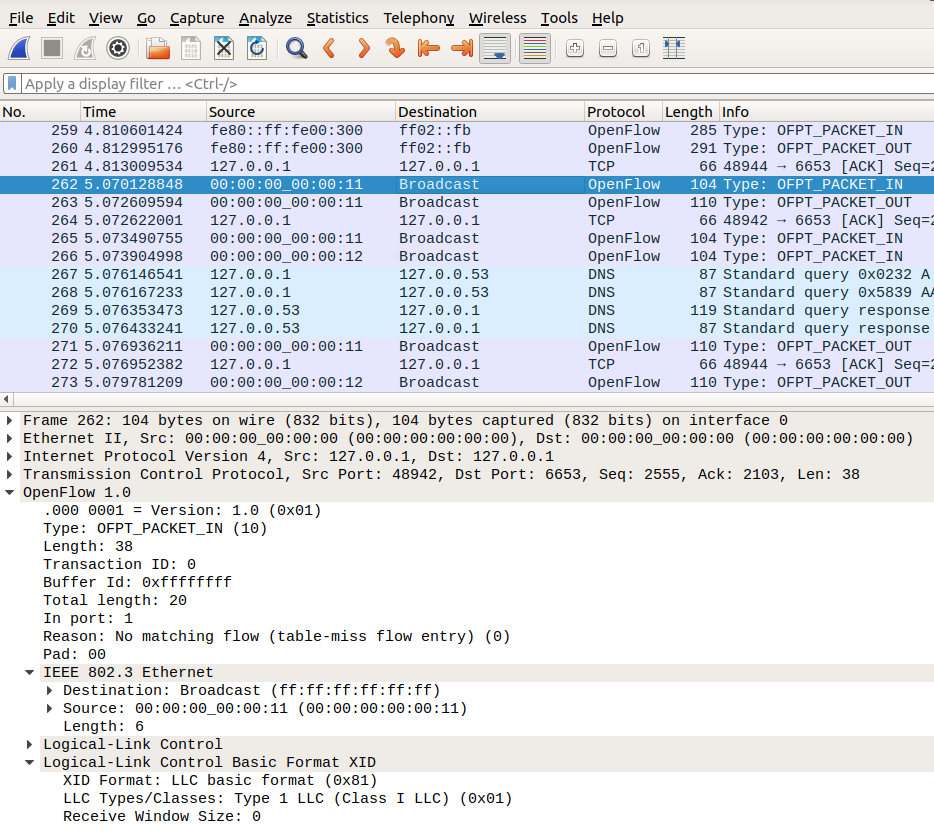
\includegraphics[scale=0.4]{Figuras/capt_1.png}
		\caption{Consulta de ap1 al controlador}
		\label{fig:capt_1}
	\end{figure}

En su respuesta, el controlador indica mediante un paquete \texttt{OFPT\_PACKET\_OUT} que ap1 debe enviar ese tipo de tráfico por el puerto 65531, comportándose como un switch normal al que le llega un paquete dirigido a la dirección de broadcast. En la Figura \ref{fig:capt_2} se muestra el paquete capturado,\par

	\begin{figure}[!h]
		\centering
		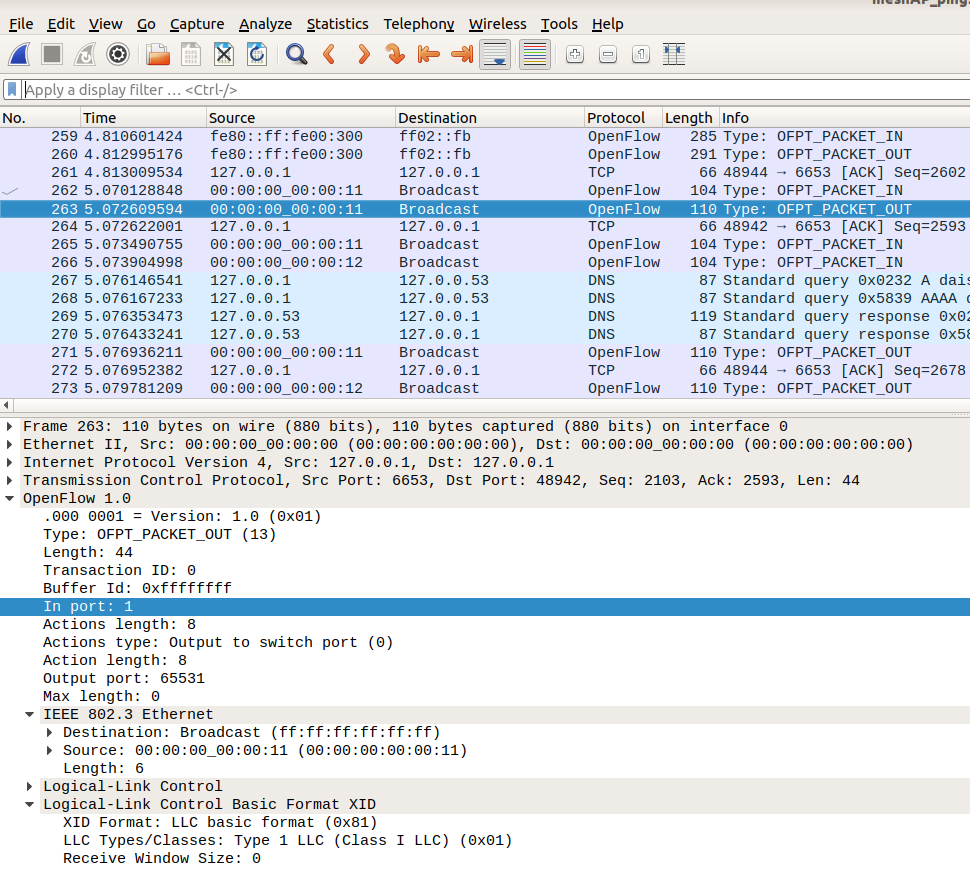
\includegraphics[scale=0.4]{Figuras/capt_2.png}
		\caption{Respuesta del controlador a ap1}
		\label{fig:capt_2}
	\end{figure}

Cuando el paquete llega a ap2 a través de ap1, ocurre lo mismo; ap2 envía una consulta al controlador mediante un mensaje \texttt{OFPT\_PACKET\_IN} para saber qué hacer con el paquete enviado por sta1 a la dirección de broadcast, que ha recibido por su interfaz ap2-mp2. El controlador contesta con un paquete \texttt{OFPT\_PACKET\_OUT} que debe expulsar el paquete pos el resto de sus puertos.\par 

Hay que destacar que en estos casos el controlador no indica a ap1 ni a ap2 que instalen entradas nuevas para este tipo de tráfico en sus tablas de flujos, sino que únicamente les indica qué debe hacer con ellos. Si se volviera a enviar un paquete desde sta1 dirigido a la dirección de broadcast, los \textit{access points} tendrían que volver a consultar al controlador.\par 

Sin embargo, en la respuesta de sta2 al \texttt{ARP request} procedente desde sta1, ocurre algo diferente. sta2 responde con un \texttt{ARP reply}, que llega a ap2, y este realiza la pertinente consulta al controlador mostrada en la Figura \ref{fig:capt_3}.\par 

	\begin{figure}[!h]
		\centering
		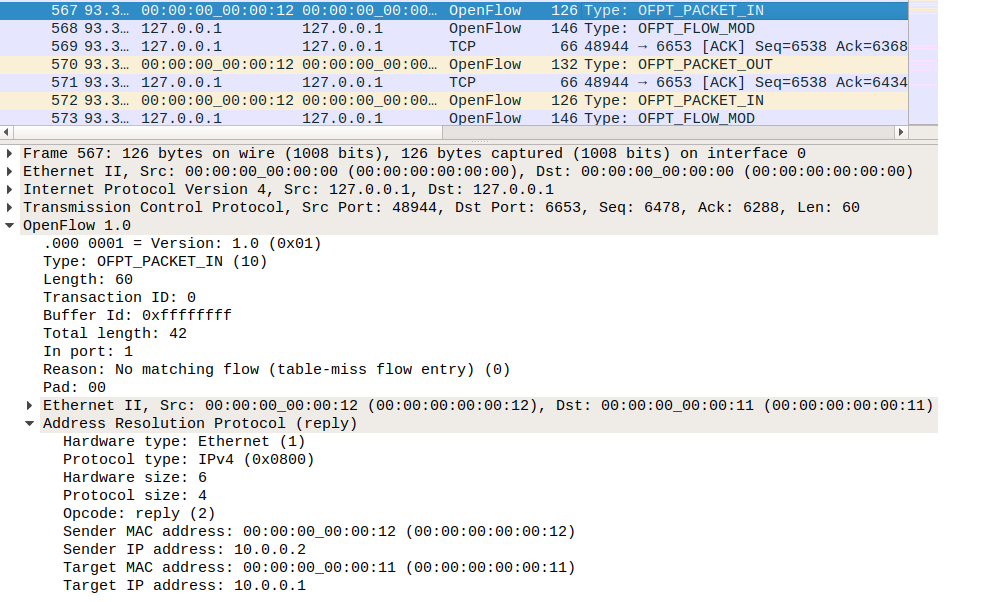
\includegraphics[scale=0.4]{Figuras/capt_3.png}
		\caption{Consulta de ap2 al controlador}
		\label{fig:capt_3}
	\end{figure}

En este caso el controlador envía dos paquetes como respuesta a la consulta de ap2. Se trata de un mensaje \texttt{OFPT\_FLOW\_MOD}, en el que indica a ap2 que debe añadir una nueva entrada a su tabla de flujos para el tráfico que se indica en el mensaje \texttt{OFPT\_PACKET\_OUT}. Las Figuras \ref{fig:capt_4} y \ref{fig:capt_5} muestran estos dos paquetes capturados. \par

	\begin{figure}[!h]
		\centering
		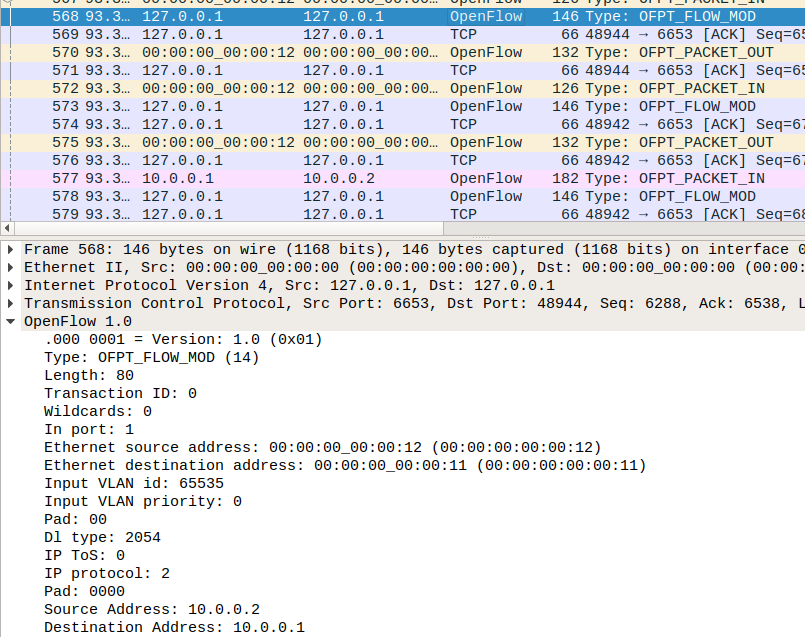
\includegraphics[scale=0.41]{Figuras/capt_4.png}
		\caption{Respuesta de modificación del controlador a ap2}
		\label{fig:capt_4}
	\end{figure}
	
	\begin{figure}[!h]
		\centering
		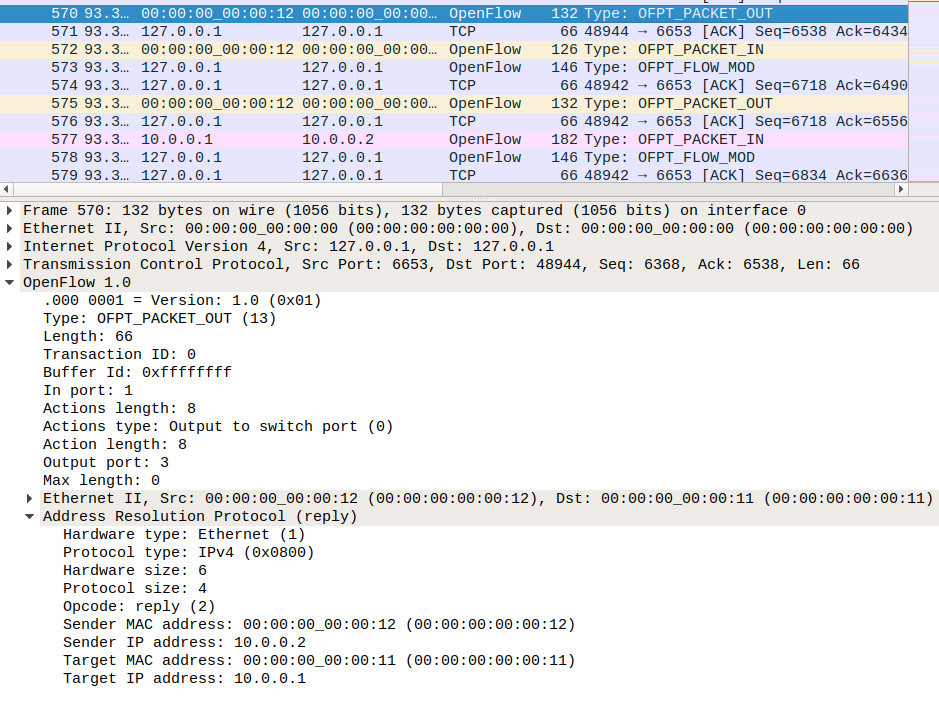
\includegraphics[scale=0.4]{Figuras/capt_5.png}
		\caption{Respuesta del controlador con las acciones a instalar en ap2}
		\label{fig:capt_5}
	\end{figure}

Por tanto, ap2 añade un nuevo flujo en su tabla para el tráfico \texttt{ARP reply} procedente de sta2 y destinado a sta1, que entra por el puerto 1 de ap2, correspondiente a la interfaz 'ap2-wlan1', para que sea enviado por el puerto 3 de ap2, interfaz 'ap2-mp2'. En ap1 ocurre lo mismo: tras su consulta al controlador para ese tipo de tráfico, este le responde con dos mensajes para que instale un nuevo flujo en su tabla.\par 

Se puede comprobar que realmente estos flujos se instalan en los \textit{access points}: mirando el listado de flujos del apartado \ref{sect:tablas_flujos} se deben encontrar estas reglas.\par

En ap1:\par 

\noindent\texttt{
	cookie=0x0, duration=5.054s, table=0, n\_packets=0, n\_bytes=0, idle\_timeout\\
	=60, priority=65535, arp,
	in\_port='ap1-mp2',vlan\_tci=0x0000,dl\_src=00:00:00:\\
	00:00:12,dl\_dst=00:00:00:00:00:11,
	arp\_spa=10.0.0.2,arp\_tpa=10.0.0.1,arp\_\\
	op=2 actions=output:'ap1-wlan1'
}

\hspace{1cm}

En ap2:\par 

\noindent\texttt{
	cookie=0x0, duration=6.802s, table=0, n\_packets=0, n\_bytes=0, idle\_timeout\\
	=60, priority=65535,
	arp,in\_port='ap2-wlan1',vlan\_tci=0x0000,dl\_src=00:00:00:\\
	00:00:12,dl\_dst=00:00:00:00:00:11,
	arp\_spa=10.0.0.2,arp\_tpa=10.0.0.1,arp\_op=2 actions=output:'ap2-mp2'
}

De igual manera, cuando sta1 envía el \texttt{ICMP echo request} hacia sta2, al llegar el paquete a la interfaz 'ap1-wlan1', ap1 consultará al controlador, como muestra la figura \ref{fig:capt_6}.\par 
	
	\begin{figure}[!h]
		\centering
		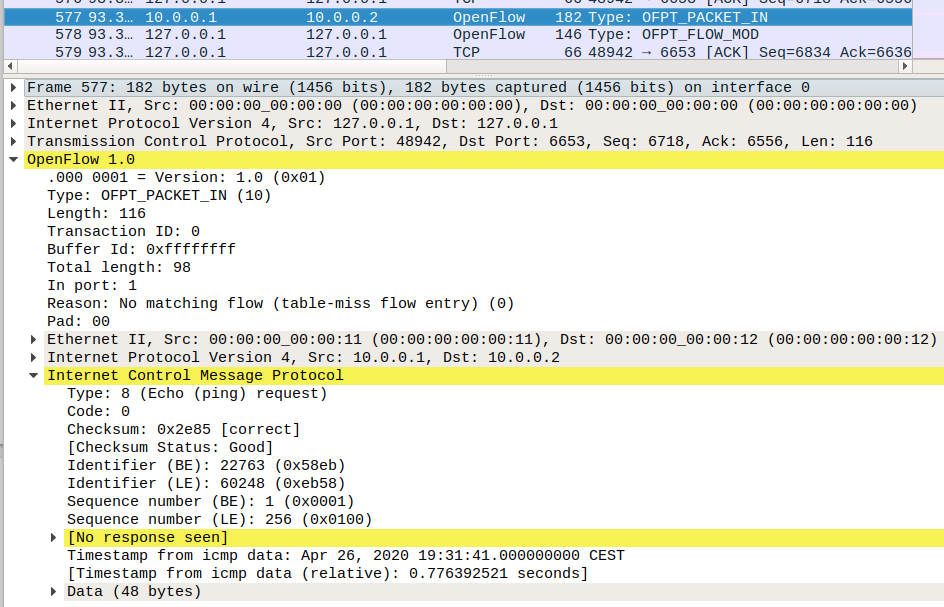
\includegraphics[scale=0.4]{Figuras/capt_6.png}
		\caption{Consulta de ap1 del \texttt{ICMP echo request}}
		\label{fig:capt_6}
	\end{figure}

Igual que en el caso anterior, el controlador contesta a ap1 indicándole que debe instalar un nuevo flujo para el tráfico \texttt{ICMP echo request} procedente de sta1 hacia sta2, que entra por el puerto 1, interfaz 'ap1-wlan1' y que debe ser enviado por el puerto 3 'ap1-mp2'. En las Figuras \ref{fig:capt_7} y \ref{fig:capt_8} se muestran estos mensajes.\par 
	
	\begin{figure}[!h]
		\centering
		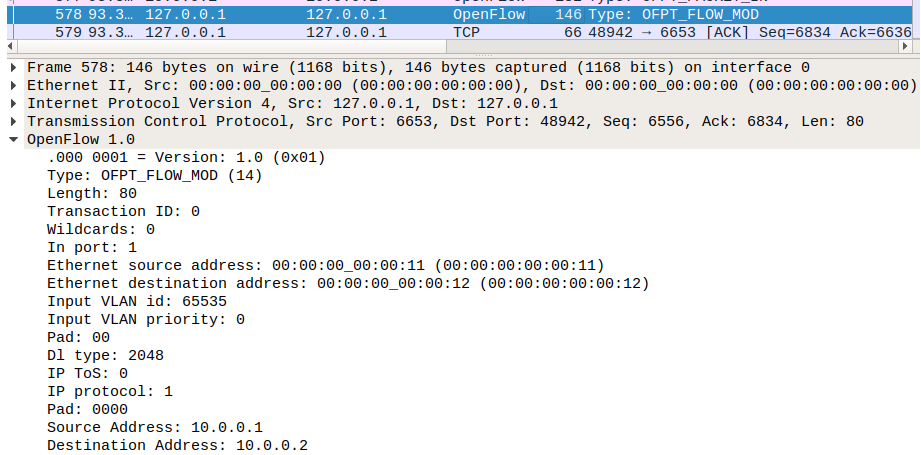
\includegraphics[scale=0.4]{Figuras/capt_7.png}
		\caption{Respuesta del controlador con la modificación del flujo en ap2}
		\label{fig:capt_7}
	\end{figure}
	
	\begin{figure}[h]
		\centering
		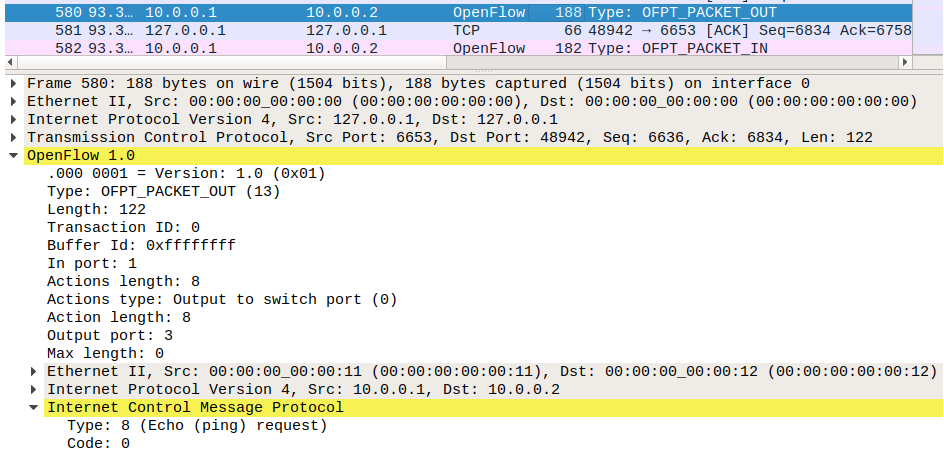
\includegraphics[scale=0.4]{Figuras/capt_8.png}
		\caption{Respuesta del controlador con las acciones a instalar en ap1}
		\label{fig:capt_8}
	\end{figure}

Los restantes flujos instalados en los \textit{access points} se añaden a las tablas de flujos de igual manera que los dos últimos casos analizados.\par 

No obstante, a parte de indicar cómo es la instalación de estos flujos, las capturas también aportan información acerca de las interfaces que se conectan entre ellas:\par 

\begin{itemize}
	\item En sta1 'sta1-wlan1' se conecta con 'ap1-wlan1'.
	\item En ap1, a parte de la conexión indicada anteriormente, 'ap1-mp2' se conecta con 'ap2-mp2'.
	\item En ap2, además de la conexión con ap1, 'ap2-wlan1' se conecta con 'sta2-wlan1'.
\end{itemize}

Con esta información de las conexiones entre los nodos es sencillo completar el esquema de la topología de la red mostrada en en el apartado \ref{sect:topo_inicial}. La topología resultante se muestra en el apartado \ref{sect:topo_completa}.\par 

\section{Topología completa resultante}\label{sect:topo_completa}

	\begin{figure}[!h]
		\centering
		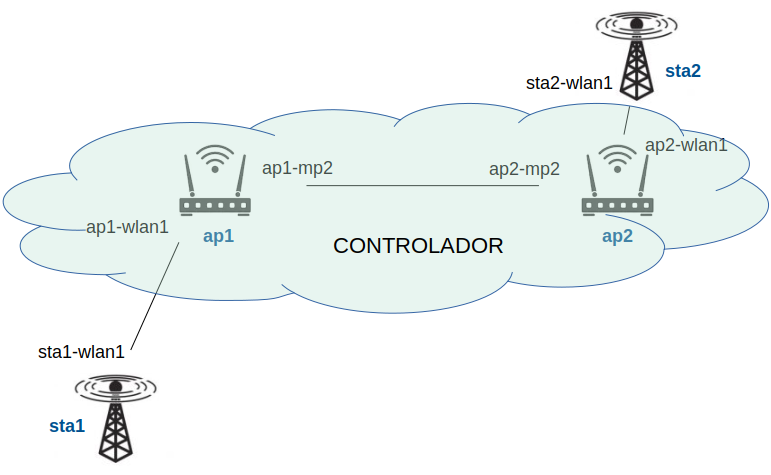
\includegraphics[scale=.4]{Figuras/topo_completa.png}
		\caption{Topología resultante de la red meshAP.}
		\label{fig:topo_completa}
	\end{figure}


\end{document}